\documentclass[10pt,letterpaper]{article}

\usepackage{cogsci}
\usepackage{pslatex}
\usepackage{apacite}

\usepackage{amsmath, amsthm, amssymb}
\usepackage{graphicx}
\usepackage{color}

\newcommand{\TODO}[1]{\textcolor{red}{[TODO: #1]}}

\newcommand{\threshold}[0]{$T=2$}
\newcommand{\betazero}[0]{$\beta_0=683.86,\ 95\%\ \mathrm{CI}\ [601.66, 766.06]$}
\newcommand{\betaone}[0]{$\beta_1=46.01,\ 95\%\ \mathrm{CI}\ [19.71, 72.32]$}
\newcommand{\betatwo}[0]{$\beta_2=63.67,\ 95\%\ \mathrm{CI}\ [57.26, 70.07]$}
\newcommand{\kapb}[0]{$\kappa_b=50.42$}
\newcommand{\kapm}[0]{$\kappa_m=502850.41$}
\newcommand{\kapv}[0]{$\kappa_v=255.60$}
\newcommand{\perr}[0]{$\sigma_p=31.02$}
\newcommand{\sdzero}[0]{$\sigma_0=167.06$}
\newcommand{\sdadj}[0]{$\sigma_{adj}=0.9$}

\newcommand{\HoleResponseCorr}[0]{$r=0.77,\ 95\%\ \mathrm{CI}\ [0.75, 0.78]$}
\newcommand{\HoleRTCorr}[0]{$r=0.67,\ 95\%\ \mathrm{CI}\ [0.64, 0.71]$}
\newcommand{\PaddleCorr}[0]{$r=0.95,\ 95\%\ \mathrm{CI}\ [0.91, 0.97]$}

\newcommand{\AvgResponse}[0]{$53.2\%$}
\newcommand{\AvgCorrect}[0]{$72.4\%$}
\newcommand{\ResponseN}[0]{$N=15216$}
\newcommand{\AvgRT}[0]{$RT=1010.13\ \mathrm{msec},\ 95\%\ \mathrm{CI}\ [997.81, 1022.74]$}
\newcommand{\ResponseFull}[0]{$\chi^2(3)=64.469,p < 0.001$}
\newcommand{\ResponseHoleClass}[0]{$\chi^2(3)=4477.182,p < 0.001$}
\newcommand{\ResponseHoleSize}[0]{$\chi^2(1)=168.598,p < 0.001$}
\newcommand{\RTFull}[0]{$\chi^2(3)=27.146,p < 0.001$}
\newcommand{\RTHoleClass}[0]{$\chi^2(3)=63.611,p < 0.001$}
\newcommand{\RTHoleSize}[0]{$\chi^2(1)=8.981,p < 0.01$}
\newcommand{\RTZeroBounces}[0]{$RT=799.99\ \mathrm{msec},\ 95\%\ \mathrm{CI}\ [783.07, 815.99]$}
\newcommand{\InterceptZeroBounces}[0]{$\beta_0=757.86,\ 95\%\ \mathrm{CI}\ [756.67, 759.05]$}
\newcommand{\RTOneBounces}[0]{$RT=1027.87\ \mathrm{msec},\ 95\%\ \mathrm{CI}\ [1007.75, 1050.46]$}
\newcommand{\InterceptOneBounces}[0]{$\beta_0=894.24,\ 95\%\ \mathrm{CI}\ [891.74, 896.63]$}
\newcommand{\RTTwoBounces}[0]{$RT=1251.20\ \mathrm{msec},\ 95\%\ \mathrm{CI}\ [1225.41, 1276.81]$}
\newcommand{\InterceptTwoBounces}[0]{$\beta_0=1025.80,\ 95\%\ \mathrm{CI}\ [1021.74, 1029.79]$}

\newcommand{\ResponseTrialCorr}[0]{$\rho=0.27,\ 95\%\ \mathrm{CI}\ [0.07, 0.45]$}
\newcommand{\ResponseTrialCorrEarly}[0]{$\rho=0.41,\ 95\%\ \mathrm{CI}\ [0.10, 0.66]$}
\newcommand{\ResponseTrialCorrLate}[0]{$\rho=-0.08,\ 95\%\ \mathrm{CI}\ [-0.38, 0.22]$}
\newcommand{\RTTrialCorr}[0]{$\rho=-0.89,\ 95\%\ \mathrm{CI}\ [-0.93, -0.84]$}
\newcommand{\RTTrialCorrEarly}[0]{$\rho=-0.88,\ 95\%\ \mathrm{CI}\ [-0.94, -0.82]$}
\newcommand{\RTTrialCorrLate}[0]{$\rho=-0.66,\ 95\%\ \mathrm{CI}\ [-0.83, -0.41]$}

\newcommand{\HoleNumFailed}[0]{$N=8$}
\newcommand{\HoleNumIncomplete}[0]{$N=25$}
\newcommand{\HoleNumOk}[0]{$N=320$}
\newcommand{\HoleNumComplete}[0]{$N=328$}
\newcommand{\PaddleNumFailed}[0]{$N=18$}
\newcommand{\PaddleNumIncomplete}[0]{$N=3$}
\newcommand{\PaddleNumOk}[0]{$N=42$}
\newcommand{\PaddleNumComplete}[0]{$N=60$}

\newcommand{\AicFull}[0]{$\mathrm{AIC}=5012$}
\newcommand{\BicFull}[0]{$\mathrm{BIC}=5024$}
\newcommand{\AicNoBounces}[0]{$\mathrm{AIC}=5276$}
\newcommand{\BicNoBounces}[0]{$\mathrm{BIC}=5284$}
\newcommand{\AicNoSamples}[0]{$\mathrm{AIC}=5032$}
\newcommand{\BicNoSamples}[0]{$\mathrm{BIC}=5040$}


% space below "Figure 1: ...", but only for inline figures
%\addtolength{\textfloatsep}{-0.1cm}

\addtolength{\abovecaptionskip}{-0.25cm}
\addtolength{\belowcaptionskip}{-0.5cm}

\title{Think again?\\ The amount of mental simulation tracks uncertainty in the outcome}

\author{{\large \bf Jessica B.~Hamrick$^1$ (jhamrick@berkeley.edu),
    Kevin A.~Smith$^2$ (k2smith@ucsd.edu),}\\
    {\large \bf Thomas L.~Griffiths$^1$ (tom\_griffiths@berkeley.edu),
      \& Edward Vul$^2$ (evul@ucsd.edu)}\\
    $^1$University of California, Berkeley, Department of Psychology, Berkeley CA 94720 USA\\
    $^2$University of California, San Diego, Department of Psychology, La Jolla, CA 92093 USA}

\begin{document}

\maketitle

\begin{abstract}
In this paper, we investigate how people use mental simulations.
In particular, do people vary the number of mental simulations that they run in order to optimally balance speed and accuracy?
To answer this question, we focused on the particular domain of intuitive physics, for which there is prior evidence that people use mental simulation to make predictions about the world \cite<e.g.>{Smith:2013fc,Battaglia2013}.
We combined a model of approximate, noisy physical simulation with a well-known strategy in decision making called the \emph{sequential probability ratio test}, or \textsc{sprt} \cite{wald1947sequential}.
Our model predicted that people should vary the number of simulations that they run depending on their own uncertainty about the outcome.
Specifically, they should use more samples when it is harder to make an accurate prediction due to higher uncertainty in their simulations.
We tested this hypothesis through a task in which people watched a ball bouncing around in a box, and had to judge whether it would first go through a hole in the wall, or bounce off that wall. 
We varied the uncertainty of each trial by changing the size of the holes and the margin by which the ball either went through the hole or missed the hole. 
Both people's judgments and their response times were well-predicted by our model, demonstrating that people have a systematic strategy to allocate their resources for mental simulation.

\textbf{Keywords:} 
mental simulation; intuitive physics; \textsc{sprt}; computational modeling
\end{abstract}

\section{Introduction}

%% The question we're interested in: how many simulations do people take?
How should the mind optimally allocate its computational resources?
Consider the game of Angry Birds, where the goal is to launch birds to knock down a tower.
To take a shot, the player can imagine---or \emph{mentally simulate}---the path the bird will take and how it will affect the tower.
How long should the player spend thinking before they let each bird fly?
If they spend no time thinking, they are likely to miss the target.
But, if they spend too long thinking, it will take much longer to receive the satisfaction of beating the level.
More generally, if running simulations will provide a more accurate forecast but incur a sampling cost, how long should an agent spend simulating before acting?

In the domain of physical reasoning, research suggests that people make predictions about physical scenes---such as those found in Angry Birds---by running noisy physical simulations \cite{Sanborn2013,Smith:2013fc,Battaglia2013,Smith:2013ug,Smith:2013th,Smith:2014tx,Ullman:2014ut,Hamrick:2015}.
However, while this research has investigated the \emph{mechanism} for making these predictions, there has been very little investigation into how people \emph{use} this mechanism. 
In particular, because the simulations are noisy, it may be beneficial to run multiple simulations in order to obtain more accurate predictions.
Is there an optimal number of simulations to run in these situations?
If so, do people behave optimally?

To investigate how many simulations people run, we focus on a dichotomous prediction task---will a ball in motion on a computer screen go through a hole, or miss it?
To model this task, we combine a mechanism of noisy physical simulation with a decision strategy for sample-based agents.
Specifically, we consider the \textit{sequential probability ratio test}, or \textsc{sprt}, in which an agent takes samples that point to one hypothesis or another, and continues to do so until the net samples in favor of one hypothesis reaches a threshold, at which point that hypothesis wins \cite{wald1947sequential}. 
Often under the name of the \emph{drift-diffusion} model, \textsc{sprt} has been used successfully to explain behavior in a number of decision-making tasks \cite<e.g.>{Gold:2007fo,Ratcliff:2008ux,Bitzer:2014ea}, as it provides an optimal cost-benefit tradeoff between sampling and exploiting information \cite{Wald:1950uw}.
Importantly, the \textsc{sprt} strategy predicts that people need to take more samples---and thus also will take a longer time to respond---when there is roughly equal evidence for both hypotheses.

\begin{figure*}[t!]
    \begin{center}
        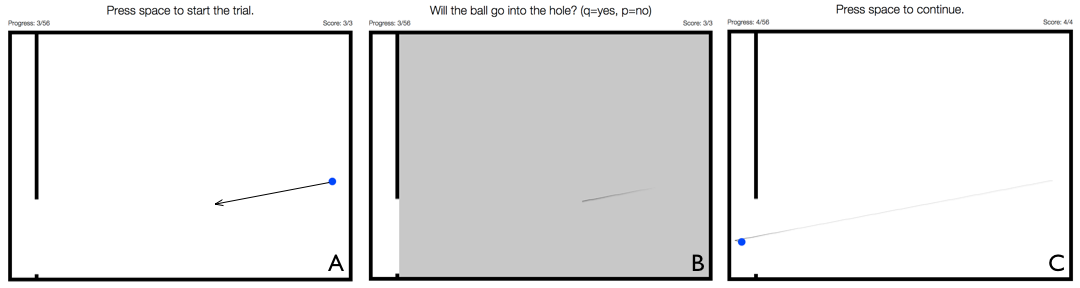
\includegraphics[width=\textwidth]{figures/experiment.png}
        \caption{\textbf{Example experimental trial.} 
        Each panel shows a different part of the trial. 
        \emph{A:} the initial screen presented to the participant.
        The arrow was not part of the actual stimuli; it has been added to reflect the animation that participants observed after pressing ``space''. 
        \emph{B:}  the screen is occluded after observing the stimulus presentation. 
        The faded gray line shows the path the ball took during the initial presentation. 
        \emph{C:} the final position of the ball, after observing the feedback. 
        As in the middle panel, the faded gray line shows the path of the ball.}
        \label{fig:experiment}
    \end{center}
\end{figure*}

%% Plan of the paper
Drawing on the results from both physical simulation and decision-making, we hypothesize that people make predictions by running mental simulations, and that they vary the number of simulations based on their uncertainty.
In this paper, we first formalize our model, combining the simulation model from \citeA{Smith:2013fc} with the \textsc{sprt} decision strategy. 
Next, we describe an experiment in which we asked participants to respond to the question of, ``will the ball go through the hole?'', and analyze peoples' judgments and response times. 
We then demonstrate that our model can explain the empirical pattern of responses and response times we observed. 
Finally, we discuss the implications of our results on the broader, underlying question: how should people optimally make use of mental simulations?

\section{Making decisions from mental simulations}

Consider the task in Figure \ref{fig:experiment}, in which people observe a ball moving inside a box, and must predict whether it will go through a hole or not.
How do people solve this problem?
In this section, we formalize a model that answers this question by combining noisy physical simulations with a decision-making strategy known as the \emph{sequential probability ratio test}, or \textsc{sprt}.

\subsection{Modeling physical simulation}

There is a growing body of evidence that people reason about physical scenes like the one in Figure \ref{fig:experiment} by running noisy simulations.
This hypothesis, referred to as the ``noisy Newton'' hypothesis \cite{Sanborn2013}, states that people have approximate knowledge of physical laws instantiated in a runnable model of intuitive physics.
Using this model, they can extrapolate the future by running a series of noisy simulations \cite{Smith:2013fc,Battaglia2013,Smith:2013ug,Smith:2013th,Smith:2014tx,Ullman:2014ut,Hamrick:2015}.

\citeA{Smith:2013fc} investigated the various sources of uncertainty in these simulations, finding that people's judgments were best captured by a model that took into account both perceptual uncertainty (noise in exactly where objects are and their motion trajectories) and dynamic uncertainty (stochastic noise added to account for unknowable variation in motion---e.g., a textured floor would cause a ball rolling along it to deviate from a straight line).
Using a model like this, we can hypothesize how people reason about the task in Figure \ref{fig:experiment}: that they run noisy physical simulations to estimate where the ball will go.

\subsection{The \textsc{sprt} strategy}

If people are running simulations to reason about physical scenes, then how many simulations do they run?
Because the simulations are noisy, it might be beneficial to run multiple simulations in order to get a better estimate of the outcome.
However, each simulation comes with a time cost.
To optimize this speed-accuracy tradeoff, we apply the \emph{sequential probability ratio test}, or \textsc{sprt} \cite{wald1947sequential} to the samples drawn from the physical simulation.
By combining these two models, we can make predictions both for people's judgments, and how long they take to make those judgments.

Formally, we consider binary (or two-alternative forced choice) decisions, where an agent must choose one of two hypotheses, $H_0$ or $H_1$.
In the case of the task in Figure \ref{fig:experiment}, we can think of $H_1$ as the hypothesis that the ball goes in, and $H_0$ as the hypothesis that it does not. 
The agent may take samples $X_i$ from a Bernoulli distribution parameterized by an unknown parameter $p$ (the probability of sampling evidence for $H_1$), and from these samples estimate the probability that $H_1$ is correct: $\hat{p}=\frac{1}{N}\sum_{i=1}^N X_i$, where $N$ is the total number of samples. 
Then, the decision rule which minimizes the probability of error is $\hat{H}(X_1,\ldots{},X_N)=H_0$ when $\hat{p}<0.5$ and $\hat{H}(X_1,\ldots{},X_N)=H_1$ when $\hat{p}>0.5$.

In the best possible case, the agent takes infinitely many samples and chooses the \emph{maximum a posteriori} (MAP) hypothesis with probability $p$. 
In practice, the agent cannot take infinitely many samples. 
Thus, to determine when to stop sampling (i.e., what the value of $N$ is), the agent continues to sample until the net evidence $Y_N$ reaches some threshold, either $Y_N=T$ to select in favor of $H_1$ or $Y_N=-T$ to select in favor of $H_0$. 
The net evidence is the sum of samples in favor of $H_1$ minus those in favor of $H_0$, or $Y_N=\sum_{i=1}^N 2X_i-1$.

Independent of the actual number of samples taken, the probability of choosing the MAP hypothesis ($H_1$) is:
\begin{equation}
\Pr[\hat{H}(Y_N)=H_1\,|\,H_1,T,p]=\frac{p^T}{p^T+(1-p)^T},
\label{eq:pr-choose-h1}
\end{equation}
and the expected number of samples taken before reaching either $Y_N=T$ or $Y_N=-T$ is given by:
\begin{equation}
\mathbb{E}[N\,|\,T,p]=\frac{T}{1-2p}-\frac{2T}{1-2p}\cdot{}\frac{1-((1-p)/p)^T}{1-((1-p)/p)^{2T}},
\label{eq:expsamp}
\end{equation}
which is derived by \citeA[ch.~XIV, eq. 3.4]{Feller:1968ut}.

\subsection{Combining simulation and \textsc{sprt}}

In order to combine simulation and \textsc{sprt}, we used the model from \citeA{Smith:2013fc} to sample possible trajectories of the ball.
We then used those trajectories to estimate a posterior predictive distribution of where the ball will go.
Specifically, this distribution was a truncated normal, with the mean and standard deviation estimated from samples from the physical simulation model.
Then, the probability $p$ that the ball goes in the hole is the probability mass overlapping the hole.
This probability can then be used to compute Equations \ref{eq:pr-choose-h1} and \ref{eq:expsamp}, which give a formal hypothesis for what decisions people make, and how long it takes them.

Because our experiment (described in the next section) was performed online, we needed to fit the parameters of the model from \citeA{Smith:2013fc} to reflect these different viewing conditions.
To do this independently of the results of the experiment in this paper, we performed an online replication of the experiment from \citeA{Smith:2013fc} in which we asked people to catch a ball like the one in Figure \ref{fig:experiment} using a paddle that could move up and down along the $y$-axis (see the Appendix for details).
However, it is possible that the participants in the auxiliary experiment used more than one sample to determine where the ball would go.
Assuming they took on average $M$ samples, then the standard deviation of their judgments ($\sigma_{judgments}$) is not equal to the standard deviation of their simulations ($\sigma_{sims}$), but is instead related by the equation: $\sigma_{judgments} = \sigma_{sims} / \sqrt{M}$.
Therefore, to estimate $\sigma_{sims}$, we allowed for a free parameter, $\sigma_{adj}=\sqrt{M}$, which multiplied our original estimate of the standard deviation.

\section{Testing the \textsc{sprt} model of mental simulation}

\begin{figure*}[t]
    \begin{center}
        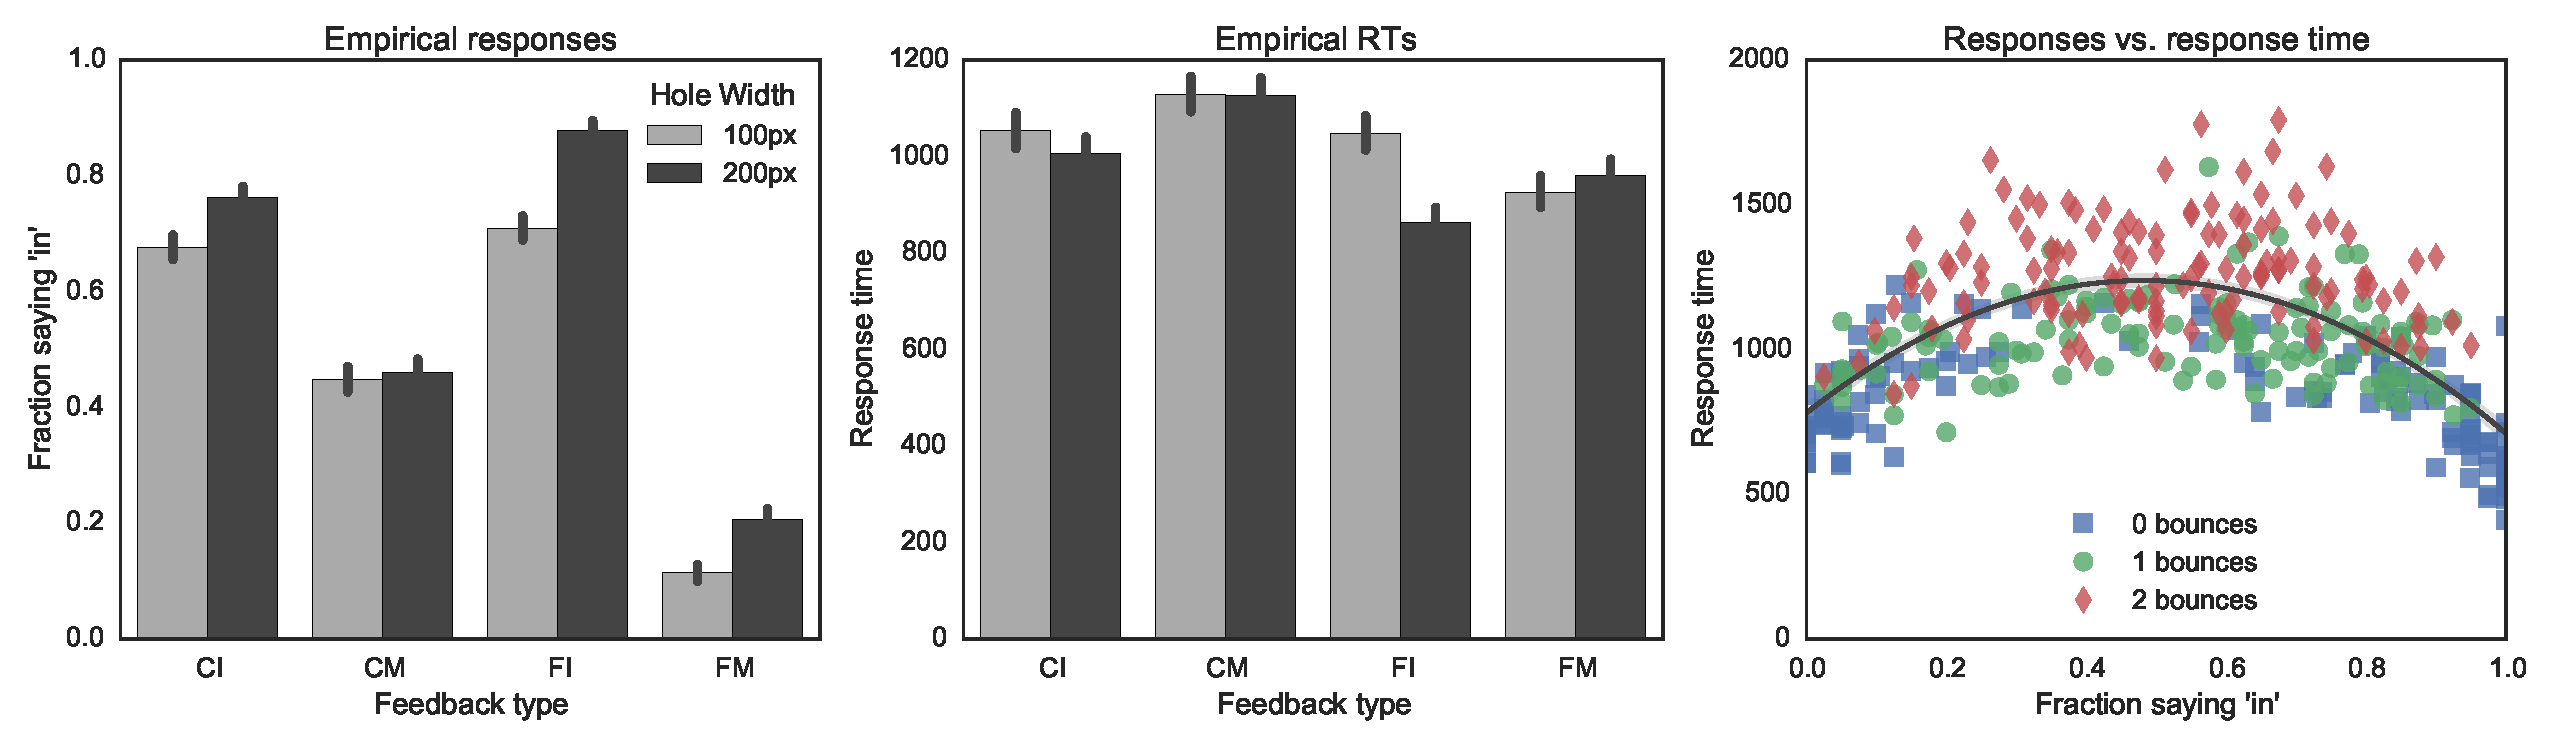
\includegraphics[width=\textwidth]{figures/hole_empirical_results.pdf}
        \caption{\textbf{Response characteristics as a function of trial type.}
        \emph{A:} each bar shows the proportion of participants saying that the ball will go in the hole for a particular trial type ($x$-axis) and hole size (color).
        \emph{B:} like the left subplot, but the $y$-axis shows bootstrapped logarithmic means of response times. 
        \emph{C:} each point corresponds to a different stimulus, trial type, and hole size.  
        The $x$-axis is the proportion of participants saying the ball will go in the hole, and the $y$-axis is the logarithmic mean response time. 
        The black line indicates a 2nd-order polynomial fit between responses and response times and the shaded gray region indicates the 95\% confidence interval around the fit.}
        \label{fig:pct-vs-rt}
    \end{center}
\end{figure*}

To determine whether people choose the number of simulations in a way consistent with \textsc{sprt}, we designed an experiment in which people made a binary judgment about what will happen in the future.
Specifically, we asked participants to reason about whether a ball traveling across a computer screen would go through a hole or not (see Figure \ref{fig:experiment}).
We designed the trials to elicit a range of responses by varying the margin by which the ball either missed or went through the hole.
According to \textsc{sprt}, people should be slower to respond on trials where, according to their simulations, the probability that the ball goes in the hole is close to $p=0.5$ (e.g., where the ball just barely goes through the hole, or just barely misses the hole), and they should be faster to respond when their simulations are more certain (e.g., where the ball goes directly through the center of a large hole, or hits the wall very far away from the hole).

\subsection{Participants}

We recruited \HoleNumComplete{} participants on Amazon's Mechanical Turk using the psiTurk \cite{McDonnell12} experimental framework.
Participants were treated in accordance with UC Berkeley IRB standards and were paid \$0.60 for approximately 6.5 minutes of work.
Participants were randomly assigned to one of eight conditions, which determined which stimuli they judged based on a latin-square design (see Stimuli). 
Additionally, we excluded \HoleNumFailed{} participants from analysis for answering incorrectly on more than one control trial (see Stimuli), leaving a total of \HoleNumOk{} participants.

\subsection{Procedure}

On each trial, participants were shown the scene, including the initial position of the ball and the location of the hole. 
Participants were instructed to press ``space'' to begin the trial. 
Immediately upon pressing ``space'', an animation of the initial stimulus began (see Stimuli). 
As soon as this animation concluded, a gray box was drawn over the screen, occluding the ball (but not the line depicting the path it had traveled so far; this was left in as a reminder to participants of where the ball had come from). 
Participants were asked, ``will the ball go in the hole?'', and were instructed to press `q' if they thought it would, and `p' if they thought it would not. 
After responding, text appeared saying ``Correct!'' or ``Incorrect.''
The gray occluder was removed, and participants were shown a feedback animation of the path of the ball (see Stimuli).
The final frame of this animation remained on the screen until participants pressed ``space'' to advance to the next trial.

During the experiment, participants made judgments on 48 experimental trials, presented in a random order, as well as eight control trials, which were shown after every seven experiment trials, also in a random order.
In addition, participants were given seven instruction trials prior to the experiment to familiarize them with the procedure.

\subsection{Stimuli}

The stimuli consisted of two animations depicting a blue ball with a radius of 10px moving in a box with dimensions 900px $\times$ 650px.
The first animation was the stimulus presentation, which had a duration of 0.775 seconds and depicted the ball moving in a particular direction.
The second animation was 1.5 seconds of feedback, and picked up immediately where the first animation left off.
The feedback showed the ball either going into the hole or bouncing off the wall that contained the hole.
Across all stimuli, the ball always traveled the same distance during the feedback animation, and could bounce on the other walls either 0, 1, or 2 times before going into the hole or hitting the wall with the hole in it.
In both animations, the ball had a velocity of 400px/s, and as it moved, it traced a gray line on the floor (see Figure \ref{fig:experiment}).

There were 48 different initial animations, equally balanced by number of bounces during feedback (16 each for 0, 1, and 2 bounces). 
For each of these initial animations, there were four different trial types and two different hole sizes, giving a total of eight versions of each stimulus. 
The four trial types were: ``far in'' (FI), where the ball went directly through the center of the hole; ``far miss'' (FM), where the ball missed the hole by a wide margin; ``close in'' (CI), where the ball just barely went through the hole; and `` close miss'' (CM), where the ball just barely missed the hole. 
The two hole sizes were 100px and 200px.

In order to ensure that participants never saw the same initial animation twice, we used a latin-square design of Initial Animation $\times$ Trial Type $\times$ Hole Size.
Thus, each participant saw each initial animation exactly once, each trial type exactly 12 times, and each hole size exactly 24 times.
This also ensured that the ball would go through the hole exactly half the time, so that participants would not be biased to respond either way based on statistical contingencies.

In addition to the 48 experimental trials, there were seven instruction trials and eight control trials, which were the same for all participants.
The control trials were designed to be extremely easy and were either of type ``straight hit'' (with a hole size of either 300px or 350px) or ``far miss'' (with a hole size of 100px).
Thus, participants saw a total of 63 trials.

\subsection{Results}

\subsubsection{Responses}

On average, participants were correct \AvgCorrect{} of the time and responded that the ball would go in the hole \AvgResponse{} of the time (\ResponseN{}), excluding catch trials.
There was a significant effect of trial type on participants' responses (\ResponseHoleClass{}) as well as a significant effect of hole size (\ResponseHoleSize{}).
Additionally, there was an interaction between trial type and hole size (\ResponseFull{}).
For three out of the four trial types, there was a significant difference between responses for the two different hole sizes (for CI, \ResponseCIttest{}; for FI, \ResponseCIttest{}; and for FM, \ResponseFMttest{}), with the exception being the CM trials (\ResponseCMttest{}).
Figure \ref{fig:pct-vs-rt}A shows responses as a function of trial type and hole size.

\subsubsection{Response times}

For all analyses of response time, we computed averages using bootstrapped logarithmic means (exponential of the mean of the log response times), using 10000 bootstrap samples.
Participants had an average response time of \AvgRT{}, excluding catch trials.
There were significant effects of both trial type (\RTHoleClass{}) and hole size (\RTHoleSize{}) on response time, as well as an interaction between trial type and hole size (\RTFull{}).
As in Figure \ref{fig:pct-vs-rt}B, hole size only had an effect in the case of the FI trials (\ResponsetimeFIttest{}; for CI, \ResponsetimeCIttest{}; for CM, \ResponsetimeCMttest{}; and for FM, \ResponsetimeFMttest{}).

\subsubsection{Effect of practice}

To check for any effect of practice on participants responses, we computed Spearman rank correlations (with 95\% confidence intervals computed from 10000 bootstrap samples) between trial number and accuracy, as well as between trial number and response time.
We found an overall effect of practice on accuracy (\ResponseTrialCorr{}), though in the second half of the experiment, this effect had disappeared (\ResponseTrialCorrLate{}).
There was also an overall effect of practice on response time (\RTTrialCorr{}), which was strong both in the first (\RTTrialCorrEarly{}) and second (\RTTrialCorrLate{}) halves of the experiment.
Future work will need to include a longer training period to alleviate these practice effects.

\subsubsection{Relationship of responses to reaction time}

\begin{figure*}[t]
    \begin{center}
        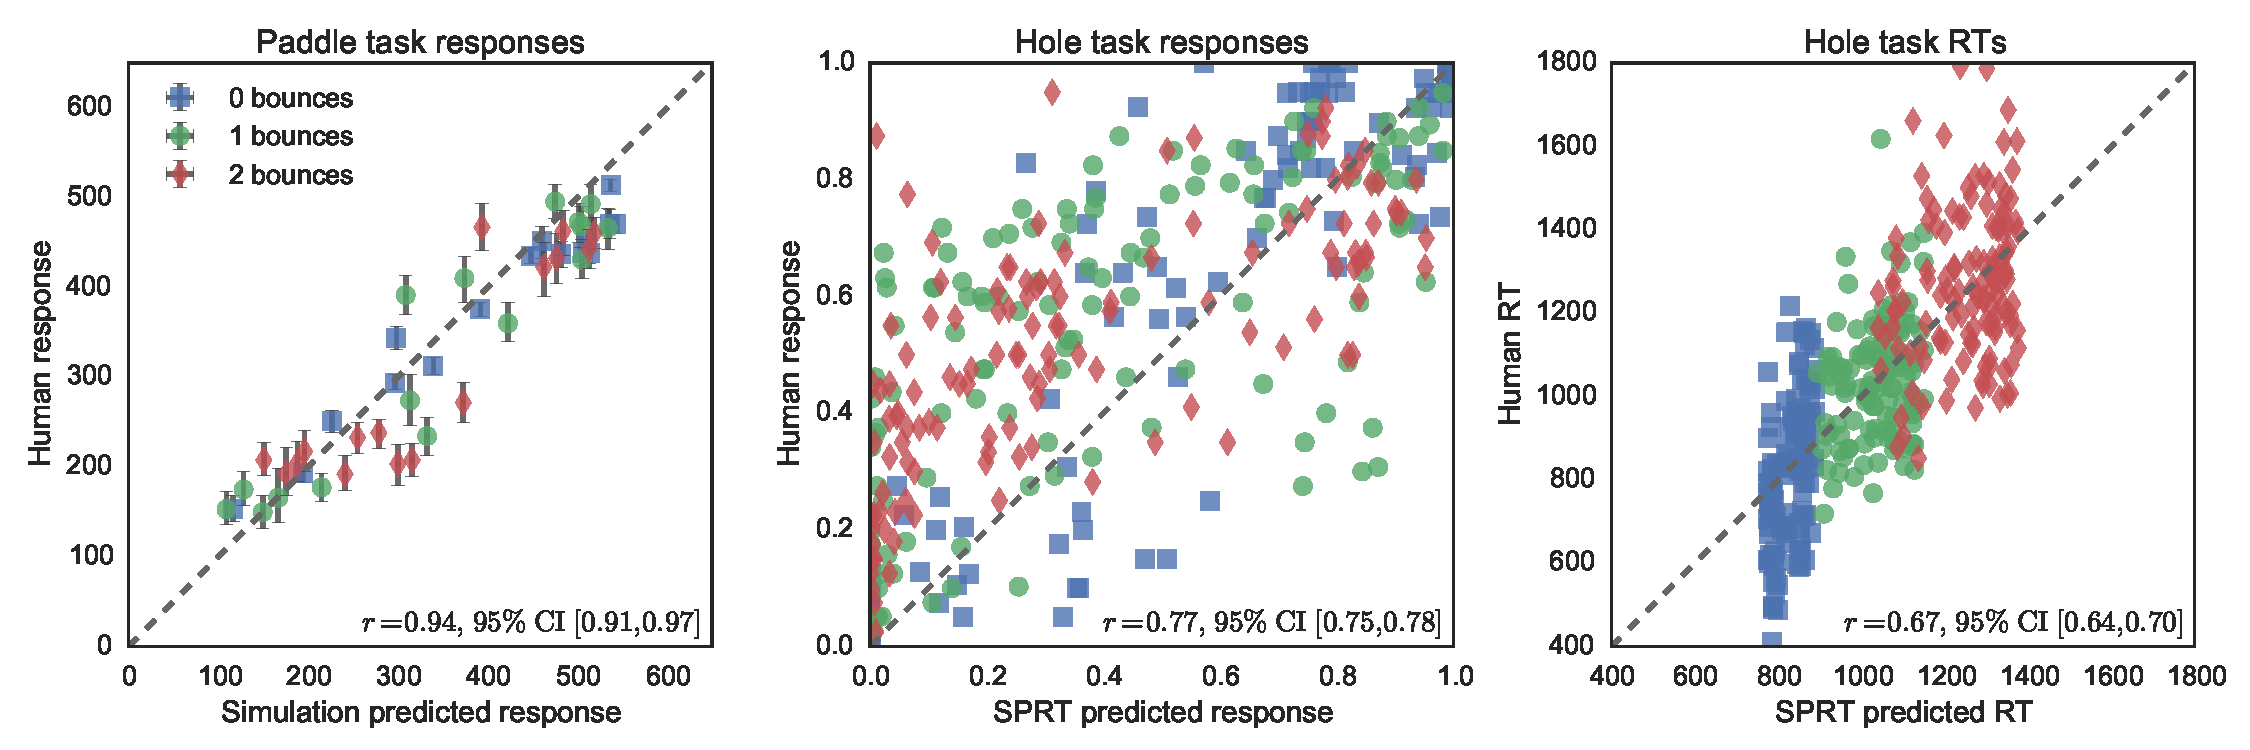
\includegraphics[width=\textwidth]{figures/model_results.pdf}
        \caption{\textbf{Model vs. human comparison.} 
        In both plots, each point corresponds to a different stimulus, trial type, and hole size. 
        Dashed lines indicate perfect correspondence between model and people. 
        \emph{A:} The $x$-axis is the probability the model says the ball will go in the hole, and the $y$-axis is the proportion of participants saying the ball will go in the hole. 
        \emph{B:} Color and shape indicate the number of times the ball bounced during feedback. 
        The $x$-axis is the model response times, and the $y$-axis is the logarithmic mean response times of participants.}
        \label{fig:model-results}
    \end{center}
\end{figure*}

As shown in Figure \ref{fig:pct-vs-rt}C, we found a clear effect of certainty on people's response times.
We fit both 1st- and 2nd-order polynomial functions to the relationship between responses and response times, and found the 2nd-order function to be a much better fit according to both AIC and BIC (for the 1st-order function, \AicFirstOrder{} and \BicFirstOrder{}; for the 2nd-order function, \AicSecondOrder{} and \BicSecondOrder{}).
These results indicate that on trials when there was more agreement amongst participants (the fraction saying `in' is closer to $0$ or $1$), participants were faster to respond than when responses were more variable.
This tradeoff mirrors the same tradeoff found in \textsc{sprt}: decisions for which $p\approx0.5$ are slower, because it on average takes more samples to get to one threshold versus the other.

In addition, we found that response time is affected by the number of bounces during feedback.
Participants were fastest to respond on trials with zero bounces (\RTZeroBounces{}), slower to respond on trials with one bounce (\RTOneBounces{}), and slowest to respond on trials with two bounces (\RTTwoBounces{}).
While this may be partially modulated by difficulty---people make more variable predictions as bounces are added \cite{Smith:2013fc}, and more variable trials have longer reaction times---there appears to be an additional time cost.
We fit a new 2nd-order polynomial function to participants' responses, and included the number of bounces as an additional regressor.
With this new model, we find that the number of bounces is a strong predictor of response time above and beyond uncertainty (with bounces, \AicSecondOrderWithBounces{} and \BicSecondOrderWithBounces{}; without bounces, \AicSecondOrder{} and \BicSecondOrder{}).
By looking at the coefficient for the number of bounces, we find that the each bounce adds approximately \RTBounceCoef{} to the overall response time.
Thus, even if people are using a \textsc{sprt}-like strategy, there is an additional time cost per bounce that cannot be explained by simulation variance alone.

\subsubsection{Model comparison}

If we assume that every sample takes the same amount of time, response times as predicted by the model should be directly proportional to $\mathbb{E}[N\,|\,T,p]$.
However, because bounces were a strong predictor of response time, our final response time equation also incorporated the number of bounces, $B$, according to $RT = \beta_0 + (\beta_1 + \beta_2\cdot{}\mathbb{E}[B]) \cdot{}\mathbb{E}[N\,|\,T,p]$.
Briefly, $\beta_0$ is the time to set up the simulation and to respond, $\beta_1$ is the time to simulate with no bounces, and $\beta_2$ is the time needed to simulate each bounce.
To compute this equation, we used the physical simulation model to determine $\mathbb{E}[B]$ as the average number of times the ball bounced across all model simulations.
We then fit all parameters ($T$, $\sigma_{adj}$, $\beta_0$, $\beta_1$, and $\beta_2$) to minimize sum squared error between modeled and observed reaction times, using 10000 samples from the physical simulation model.
The best fitting values were: \threshold{}, \sdadj{},\footnote{If \sdadj{}, then $M<1$. How could people be taking fewer than one sample?
We suspect that $\sigma_{adj}<1$ because the model actually overestimates the standard deviation; thus, $\sigma_{adj}$ is also adjusting for the inflated uncertainty in the model, and people are taking approximately one sample to catch the ball.} \betazero{}, \betaone{}, and \betatwo{}.

We computed Pearson correlations between the model and people with 95\% confidence intervals computed from 10000 bootstrap samples. The fitted model explains participants' judgments of whether the ball would go in the hole very well (\HoleResponseCorr{}, see Figure \ref{fig:model-results}A), and can additionally account for how quickly participants responded to trials (\HoleRTCorr{}, see Figure \ref{fig:model-results}B).
Even if the number of bounces is not included, the \textsc{sprt} model with \threshold{} is able to account for a moderate amount of the variance in response times (\NoBouncesHoleRTCorr{}).

A model that takes only one sample each time (equivalent to \textsc{sprt} with $T=1$) does slightly better at explaining people's responses (\RawHoleResponseCorr{}) and about as well at explaining RT (\NoSamplesHoleRTCorr{}) as the full model.
However, this model cannot explain the variation of RT within bounces, while the full model can.
For the model with $T=1$, the correlation of RT for zero bounces was \NoSamplesHoleRTCorrZeroBounces{}; for one bounce, it was \NoSamplesHoleRTCorrOneBounce{}; and for two bounces, it was \NoSamplesHoleRTCorrTwoBounces{}.
In contrast, for the model with $T=2$, the correlation of RT for zero bounces was \HoleRTCorrZeroBounces{}; for one bounce, it was \HoleRTCorrOneBounce{}; and for two bounces, it was \HoleRTCorrTwoBounces{}.
The model with $T=1$ also fares slightly worse overall according to both BIC and AIC (for $T=1$, \BicNoSamples{} and \AicNoSamples{}; for $T=2$, \BicFull{} and \AicFull{}).

\section{Discussion}

In this paper, we asked the question: do people optimally use mental simulations?
We hypothesized that people use noisy physical simulations to predict whether a ball would go in a hole, and that they vary the number of simulations in order to exploit the fact that some judgments are easier to make than others.
The results of our experiment paint a clear picture that people \emph{do} vary the number of samples they take, as evidenced by the increase in response time on the trials they were most uncertain about.
Comparing people's responses and response times to those of the model, we found an extremely strong fit.
This provides evidence that people not only rely on approximate physical simulations, but that they optimally vary the number of simulations that they run according to \textsc{sprt}.

If \textsc{sprt} is the optimal strategy, then what is the optimal threshold?
We found the best fitting \textsc{sprt} threshold to be \threshold{}, which is consistent with previous research.
According to \citeA{Vul:2014ba}, a sample-based agent should only take a small number of samples before making a judgment so long as there is any cost to taking samples.
While taking a small number of samples clearly provides a worse chance of making a good decision than taking multiple samples, over the long run, this strategy maximizes expected utility across a large number of judgments.
There has been some evidence that this story also holds true for mental simulations.
For example, \citeA{Battaglia2013} analyzed the variability of people's responses in tasks concerning towers of building blocks, and found that participants seemed to use between three and seven samples per judgment.
However, this paper is the first to provide evidence not only that people use a small number of simulations, but that they systematically vary the number of simulations rationally in response to task demands.

Mental simulation is a powerful and flexible tool, as it offers us a way to make predictions about scenarios that have not yet come to pass, or which may never come to pass.
In this work, we demonstrated that when people use mental simulation, they are sensitive to their own uncertainty in reasoning about the task and accordingly adjust how many simulations they run.
This results joins others \cite<e.g.>{Hamrick:2014wq} in explaining not just \emph{that} people use simulation to reason about the world, but specifically \emph{how} they use it.
While there are still many questions left unanswered---e.g., how do people use simulations in non-binary tasks?---this work brings us one step closer to understanding of how mental simulation is used.

\section{Appendix: Replication of \citeA{Smith:2013fc}}

\subsubsection{Participants}

We recruited \PaddleNumComplete{} participants on Amazon's Mechanical Turk using the psiTurk \cite{McDonnell12} experimental framework.
Participants were treated in accordance with UC Berkeley IRB standards and were paid \$0.60 for approximately 5 minutes of work.
Additionally, we excluded \PaddleNumFailed{} participants from analysis for failing to catch the ball on more than one control trial, leaving a total of \PaddleNumOk{} participants.

\subsubsection{Stimuli}

The stimuli were modified versions of those used the main experiment, with two differences.
First, instead of a wall with a hole in it, there was a paddle of length 100px that could move up and down the $y$-axis.
Second, instead of a full feedback animation, we just displayed the last frame of the animation.
Because there was no hole that could vary by trial, there were only 48 stimuli, plus the seven instruction trials and eight catch trials.

\subsubsection{Procedure}

The experiment was divided into two phases: the training phase (consisting of seven trials), and the experimental phase (consisting of the 48 experimental trials, with the eight control trials evenly interspersed).
On each trial, participants were shown the scene, including the initial position of the ball and the location of the hole.
The paddle begin at the center of the $y$-axis, and was freely movable along the $y$-axis from the very beginning of the trial.
Participants were instructed to press ``space'' to begin the trial and display the stimulus presentation animation.
After the stimulus presentation, a gray occluder appeared, as well as a timer that began counting down for 2 seconds.
During this time, participants had to move the paddle to try to catch the ball in the position it would be when the timer was up.
When the timer countdown finished, the paddle froze at its current location, and the occluder was removed and the full path of the ball revealed.
If the ball was on the paddle, then participants were told, ``You caught the ball!''.
If the ball was not on the paddle, participants were told ``Oops, you didn't catch the ball.''
Participants were then instructed to press ``space'' to begin the next trial.

\subsubsection{Results}

We fit the model parameters of $\sigma_p$, $\kappa_v$, $\kappa_m$, $\kappa_b$, and $\sigma_0$ to participant's responses \cite<for details, see>{Smith:2013fc}, finding the best fitting parameters to be \perr{}, \kapv{}, \kapm{}, \kapb{}, and \sdzero{}. 
With these parameters, we found very similar results to those from \citeA{Smith:2013fc}.
In particular, we found a correlation of \PaddleCorr{} between the model's predicted means of where the ball would end up and people's average location of the paddle.

\bibliographystyle{apacite}

\setlength{\bibleftmargin}{.125in}
\setlength{\bibindent}{-\bibleftmargin}

\bibliography{references}

\end{document}
